\scanpage{171}\mspage{26}
ceci de supposer que $X$ est ``localement homotopiquement trivial'', ce qui assure que le pro-ensemble simplicial que lui associent Artin-Mazur (par le procédé de nerfs de \unsure{'|''}hyperrecouvrements) est essentiellement constant dans la catégorie homotopique ordinaire - donc $X$ définit un type d'homotopie habituel. Ce n'est \uline{pas} le cas bien sur pour le topos étale d'un schéma, Pour un tel cas, le $n$-groupoïde fondamental doit être conçu comme un \uuline{pro}-$n$-groupoïde (rien d'étonnant à cela, vu la théorie familière \unsure{du|des} $\pi_1$) ; et $\unsure{\mathcal E|E}_n$ comme une $(\mathrm{ind})$-$n$-catégorie (\unsure{le|la} ind-structure correspondant à l'exigence de locale trivialité, pour un $n$-champ variable, relativement à des recouvrements de plus en plus fins de $X$\unsure{.}).

\figure{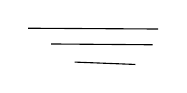
\begin{tikzpicture}[x=1cm,y=1cm]
\draw (0,0)--(1.65,-.01);
\draw (.29,-.20)--(1.58,-.21);
\draw (.59,-.43)--(1.36,-.46);
\end{tikzpicture}}

Je comprends cependant ta résistance instinctive à concevoir ce dépouillement extrême d'un beau topos $X$, au point de n'en retenir que le maigre type d'homotopie.\margin{\figure{\begin{tikzpicture}[x=1cm,y=1cm]\draw[line width=.45pt] (0,0)--(.16,.03);\end{tikzpicture}}} Bien plus, je suis persuadé qu'en\margin{\figure{\begin{tikzpicture}[x=1cm,y=1cm]\fill (0,0) circle[radius=.018];\end{tikzpicture}}}
% The short right-margin stroke is physically above the line-end hyphen in manuscript L22, bbox [1644,2129,1662,2135]. It is not assigned a verbal meaning.
% The isolated bottom-right point is physically below/right of qu'en, near [1621,2326]. Its ink-versus-reproduction status is unresolved; it is reproduced as a nontext mark, not sentence punctuation.
% archive sheet number: 171
